\documentclass[journal,twocolumn]{IEEEtran}

% -----------------------------------------------------------------------
% PACKAGES
% -----------------------------------------------------------------------
\usepackage{amsmath,amssymb,amsthm}
\usepackage{graphicx}
\usepackage{booktabs}
\usepackage{array}
\usepackage{cite}
\usepackage{url}
\usepackage{hyperref}
\usepackage{xcolor}
\usepackage{microtype}
\usepackage{siunitx}
\usepackage{multirow}

\hypersetup{
  colorlinks=true,
  linkcolor=blue!60!black,
  citecolor=blue!60!black,
  urlcolor=blue!60!black
}

% -----------------------------------------------------------------------
% THEOREM-LIKE ENVIRONMENTS
% -----------------------------------------------------------------------
\newtheorem{remark}{Remark}
\newtheorem{definition}{Definition}

% -----------------------------------------------------------------------
% CUSTOM COMMANDS
% -----------------------------------------------------------------------
\newcommand{\vx}{\mathbf{x}}
\newcommand{\va}{\mathbf{a}}
\newcommand{\vz}{\mathbf{z}}
\newcommand{\Rphase}{\mathcal{R}_{\!\phi}}
\newcommand{\patk}{p_{\mathrm{atk}}}
\newcommand{\hobs}{h(\vz)}
\newcommand{\Eref}{E_{\mathrm{ref}}}
\newcommand{\phiref}{\phi_{\mathrm{ref}}}
\newcommand{\Ntr}{N_{\mathrm{tr}}}
\newcommand{\taue}{\tau_{e}}
\newcommand{\kap}{\kappa}
\newcommand{\gam}{\gamma}
\newcommand{\dOmega}{\delta\omega}
\DeclareMathOperator*{\argmin}{arg\,min}

% -----------------------------------------------------------------------
% DOCUMENT
% -----------------------------------------------------------------------
\begin{document}

\title{Physics-Constrained Attack Search and Drift Monitoring for\\
       Optical-Injection-Locked Twin-Field QKD:\\
       A Simulator Study}

\author{%
  Mithil~Hardik~Astik%
  \thanks{M.~H.~Astik is with the Department of Physics and Electronics \&
          Electrical Engineering, BITS Pilani Hyderabad Campus, Hyderabad~500078,
          India (e-mail: f20240923@hyderabad.bits-pilani.ac.in). Manuscript received
          \today.}%
}

\markboth{IEEE Transactions on Information Forensics and Security}%
         {Astik: Physics-Constrained Search and Drift Monitoring in OIL TF-QKD}

\maketitle

% -----------------------------------------------------------------------
% ABSTRACT
% -----------------------------------------------------------------------
\begin{abstract}
Machine learning~(ML) monitors for optical-injection-locked~(OIL) twin-field
quantum key distribution~(TF-QKD) have been proposed as a practical countermeasure
against reference-beam attacks, including fast intensity modulation~(FIM) and
trojan-wavelength injection~(TWIRL). This simulator study examines supervised
monitoring under regime-held-out parameter changes, a bounded physical-parameter
search, and a nominal-model phase-residual monitor. The benchmark contains 7{,}500
windows from 750 simulated trajectories. However, the current Split C construction
reuses nominal trajectory groups in both training and test, so its reported metrics
are not leakage-free and are not interpreted as held-out generalisation. In a
200-evaluation NSGA-II search against the Split A XGBoost model, the minimum observed
attack scores were $0.887$ for FIM and $0.996$ for TWIRL; neither fell below the
reported Split A threshold of $0.038$. These are observations from evaluated
candidates, not evidence of robustness over the parameter domain. Under the specified
simulated drift conditions and the currently reported thresholds, the supervised
models produced a $100\%$ observed FPR; threshold-dependent metrics remain pending
recalculation.
The current PIAD uses the nominal phase equation; the available evaluation reports
condition-level residual values but does not document a calibrated alarm threshold
or trajectory-level FPR/TPR. Its finite-difference residual may be
dominated by coarse output sampling, and its access to simulated carrier state $N$
does not establish hardware observability. The deterministic nominal simulator,
unmodelled measurement noise, Split C overlap, and simplified TWIRL phase injection
limit interpretation of all reported results. No hardware robustness or QKD security
claim is made.
\end{abstract}

\begin{IEEEkeywords}
Twin-field QKD, optical injection locking, adversarial machine learning,
physics-informed anomaly detection, side-channel detection, simulated drift.
\end{IEEEkeywords}

% -----------------------------------------------------------------------
% I. INTRODUCTION
% -----------------------------------------------------------------------
\section{Introduction}
\label{sec:intro}

Twin-field quantum key distribution~(TF-QKD) extends the reach of secure key
exchange beyond the repeaterless rate-distance limit by exploiting single-photon
interference at an intermediate, untrusted node~\cite{lucamarini2018,wang2018}.
In deployed implementations, optical injection locking~(OIL) can be used to
establish a shared phase and frequency reference between Alice and Bob by locking
their independent slave lasers to a common reference beam~\cite{pirandola2020,
roberts2017}. This architecture introduces an externally reachable optical path:
an adversary with access to the reference path can execute physically plausible
manipulations that alter source behavior without necessarily triggering conventional
power monitoring~\cite{juarez2026}.

Juárez~\emph{et al.}~\cite{juarez2026} experimentally characterized two relevant
threats. In a \emph{fast intensity modulation}~(FIM) attack, the reference amplitude
is sinusoidally modulated at a frequency $f_\mathrm{fim}$ between
\SI{100}{\mega\hertz} and \SI{10}{\giga\hertz} with a modulation depth
$m \in [0.05, 0.40]$. In a \emph{trojan-wavelength injection}~(TWIRL), an additional
optical component is introduced at a detuned wavelength, perturbing the locked
source while potentially escaping monitoring restricted to the nominal reference
band. These mechanisms motivate software-based monitoring that operates on optical
telemetry while remaining complementary to physical isolation and filtering.

Machine-learning-based monitoring of QKD implementations has been explored across
several attack classes and device settings~\cite{baliuka2023,almohammed2021,tunc2023,
du2022,luo2022,ding2023mads,xu2024mlqkd,liu2025}. For the specific OIL-TF-QKD setting,
the baseline study in~\cite{basepaper} evaluates XGBoost and Random Forest on a
five-dimensional simulated telemetry representation and reports strong performance
under a random train-test split. That work also studies benign drift and a limited
FIM evasion search.

Two methodological questions remain central. First, random splitting does not test
generalisation to operating conditions excluded from training. Second, the meaning
of an apparent detector margin is unclear unless the adversary is constrained to
physical controls. We therefore evaluate regime-held-out data within the baseline
simulator and search the physical attack parameters. The current attack-configuration
split is not leakage-free because its nominal trajectory groups occur in both
partitions; its metrics are reported for auditability but are not used as evidence of
generalisation.

The central question is: \emph{within this simulator, what attack scores and
phase-residual behavior are observed for the specified FIM and TWIRL controls and
parameter ranges?} The phase-impact proxy is phase-derived and correlated with monitor
features; it is not treated as an independent or QKD-level impact measure. We make the
following scoped contributions:

\begin{enumerate}
  \item \textbf{Simulator benchmark and audit.} We generate 7{,}500 labeled
    simulation windows and define random-grouped and operating-regime-held-out
    evaluations. We identify and disclose nominal-group overlap in the present
    attack-configuration split (Section~\ref{sec:benchmark}).

  \item \textbf{Multi-objective physical-parameter search.} We use an offline
    score oracle and the NSGA-II multi-objective evolutionary algorithm with
    200 simulator evaluations per attack family and report the evaluated set in the
    joint space of attack score and a correlated phase-impact proxy
    (Section~\ref{sec:attack}).

  \item \textbf{Nominal-model phase-residual detector.} We evaluate a detector
    grounded in the mean-squared finite-difference residual of the Lang-Kobayashi
    phase equation. It requires no labeled attack training; the available
    condition-level residuals do not distinguish the studied FIM case, and no
    thresholded detection metric is established
    (Section~\ref{sec:piad}).
\end{enumerate}

All findings are presented within a strictly simulator-only scope. The results should
not be interpreted as evidence of hardware-level robustness, exploitability, or
composable QKD security.

% -----------------------------------------------------------------------
% II. RELATED WORK
% -----------------------------------------------------------------------
\section{Related Work}
\label{sec:related}

\subsection{OIL Reference-Beam Attacks}

Juárez~\emph{et al.}~\cite{juarez2026} experimentally established FIM and TWIRL as
relevant implementation-security threats for OIL-based TF-QKD. Their work shows that
manipulating an untrusted reference beam can alter the emitted source statistics or
introduce an out-of-band optical component that is difficult for conventional
monitoring to observe. We take this physical threat model as the starting point and
study the robustness of software-based monitoring under simulated attack and drift
conditions.

\subsection{ML-Based Security Monitoring for QKD}

Machine-learning-based QKD monitoring spans supervised classification, anomaly
detection, and attack-specific defenses~\cite{baliuka2023,almohammed2021,tunc2023,
du2022,luo2022,ding2023mads,xu2024mlqkd,liu2025}. In the OIL-TF-QKD setting,~\cite{basepaper}
introduced a five-feature telemetry representation and evaluated XGBoost and Random
Forest models, including a drift-hardened training procedure. Our study retains the
basic simulator-and-classifier setting of~\cite{basepaper} but changes the evaluation
protocol by separating operating-regime generalisation from attack-range
extrapolation and by explicitly searching over physical attack parameters.

\subsection{Adversarial Robustness in Physical Systems}

Physical-process-constrained adversarial search has been studied in cyber-physical
and optical monitoring settings~\cite{deng2017,papernot2016,peng2023}. A key
methodological principle is that the adversary should perturb controllable physical
variables and allow the governing process to determine the resulting telemetry,
rather than directly perturbing classifier features. We apply that principle here to
an OIL laser model governed by the Lang-Kobayashi equations~\cite{lang1980}. Prior
process-control security work has examined physical-process-aware detection and
response under stealthy attacks~\cite{cardenas2011,urbina2016}.

\subsection{Physics-Informed and Residual-Based Detection}

Physics-informed neural networks~(PINNs) encode differential-equation residuals as
soft constraints during learning~\cite{raissi2019}. Residual-based monitoring has
also been explored for governed physical systems~\cite{cai2021,ritto2021}. Our PIAD
is conceptually related but does not train a neural surrogate: it directly compares a
finite-difference derivative of the observed phase with the prediction of a fixed
nominal LK equation. Observer-based residual methods and stateful CUSUM-style
detectors provide relevant baselines for future matched-input comparisons
~\cite{chowdhury2020,urbina2016}.

% -----------------------------------------------------------------------
% III. SYSTEM AND THREAT MODEL
% -----------------------------------------------------------------------
\section{System and Threat Model}
\label{sec:model}

\subsection{Lang-Kobayashi Rate Equations}

We model the injection-locked slave laser at Alice's site using the
Lang-Kobayashi~(LK) rate equations~\cite{lang1980}:
\begin{align}
  \frac{dE}{dt}   &= \tfrac{1}{2}(G-\gam)E + \kap\Eref\cos(\phiref - \phi), \label{eq:E} \\
  \frac{d\phi}{dt} &= \frac{\alpha}{2}(G-\gam) - \dOmega
                      + \kap\frac{\Eref}{E+\varepsilon}\sin(\phiref - \phi), \label{eq:phi} \\
  \frac{dN}{dt}   &= I - \frac{N}{\taue} - GE^2, \label{eq:N}
\end{align}
where $E$ and $\phi$ are the intra-cavity field amplitude and phase, $N$ is the
carrier number, $G = g_0(N-\Ntr)/\Ntr$ is the modal gain, and the remaining
parameters are listed in Table~\ref{tab:params}. The equations and nominal
parameters follow the simulator basis described in~\cite{juarez2026,basepaper};
they define the present numerical model and are not a validated laser implementation.

\begin{table}[t]
  \centering
  \caption{Lang-Kobayashi Simulator Parameters}
  \label{tab:params}
  \renewcommand{\arraystretch}{1.15}
  \begin{tabular}{@{}lll@{}}
    \toprule
    Symbol & Description & Value \\
    \midrule
    $\kap$       & Injection coupling rate        & \SI{1e9}{s^{-1}} \\
    $\alpha$     & Linewidth-enhancement factor   & $3.0$ \\
    $\dOmega$    & Nominal angular-frequency detuning & \SI{0}{s^{-1}} \\
    $\gam$       & Cavity decay rate              & \SI{1e11}{s^{-1}} \\
    $g_0$        & Linear gain coefficient        & \SI{1.2e11}{s^{-1}} \\
    $\Ntr$       & Transparency carrier number    & $10^{8}$ \\
    $\taue$      & Carrier lifetime               & \SI{1}{ns} \\
    $I_0$         & Nominal injection current      & \SI{2.0e17}{s^{-1}} \\
    $\varepsilon$& Regularisation constant        & $10^{-12}$ \\
    \bottomrule
  \end{tabular}
\end{table}

Each simulation spans $t \in [0,\,\SI{1}{\micro\second}]$ with 1{,}000 uniformly
spaced evaluation points, integrated with a BDF adaptive-step solver (relative
tolerance $10^{-3}$, absolute tolerance $10^{-6}$). Benign electrical variation is
modelled as
\begin{equation}
I(t)=I_0\left[1+0.01\sin(2\pi\times10^5 t)\right],
\end{equation}
representing the deterministic current ripple used by the simulator. The output
spacing is approximately \SI{1}{\nano\second}, whereas $\gamma^{-1}$ is
\SI{10}{\pico\second}; thus the saved phase trace does not resolve the fastest
nominal timescale. Phase-estimation noise, spontaneous-emission noise, detector
noise, bandwidth limits, quantization, and phase-unwrapping errors are not modeled.
The resulting finite-difference residual must therefore be interpreted as a
coarse-grid numerical quantity, not a validated real-time detector statistic.

\subsection{Monitor Feature Vector}

The ML monitor receives five telemetry features per non-overlapping 100-point
observation window:
\begin{equation}
  \vx = \bigl[\mu,\;\sigma^2,\;P_{sb},\;\Delta\phi,\;Q_{\mathrm{proxy}}\bigr]^{\!\top},
\end{equation}
where
\begin{align*}
  \mu       &= \mathbb{E}[|E|^2], \\
  \sigma^2  &= \mathrm{Var}[|E|^2], \\
  P_{sb}    &= \sum_{k \notin \mathcal{K}_\mathrm{dc}} |\hat{E}(f_k)|^2, \\
  \Delta\phi &= \sqrt{\mathbb{E}[(\phi-\bar{\phi})^2]}, \\
  Q_{\mathrm{proxy}} &= 0.01 + 0.1\,\Delta\phi
               + 0.05\,\sigma^2/(\mu+\varepsilon).
\end{align*}
The last quantity is a synthetic QBER \emph{proxy} inherited from the simulator
feature construction rather than a protocol-level QBER estimate. It is a deterministic
function of $\mu$, $\sigma^2$, and $\Delta\phi$, so the five-coordinate vector has
only four independent components. The subscript
$\mathcal{K}_\mathrm{dc}$ denotes the five lowest and five highest spectral bins,
excluded from $P_{sb}$ to suppress DC and aliasing artefacts.
The carrier state $N$ is used by PIAD below but is not one of these five classifier
features; the present simulator therefore gives PIAD access to a state variable whose
hardware observability has not been established.

\subsection{Physical Impact Observable}

We report an exploratory \emph{phase-impact proxy}, defined as the peak-to-peak
phase excursion over one observation window:
\begin{equation}
  \hobs \triangleq \max_{t\in W}\phi(t) - \min_{t\in W}\phi(t),
  \label{eq:impact}
\end{equation}
where $W$ denotes the window's time indices. This quantity is not independent of the
classifier inputs: it and $\Delta\phi$ and $Q_{\mathrm{proxy}}$ are phase-derived.
Consequently, their co-variation cannot establish a trade-off between monitor score
and an independent physical impact. The proxy is not a direct measure of source-power
change, QKD secure-key-rate degradation, or composable security impact.

\subsection{Threat Model}
\label{sec:threat}

We use a \textbf{simulator-side score-query} abstraction for the optimization,
formalised as follows; the study does not demonstrate that such score queries are
available to an attacker probing a live system.

\begin{definition}[Simulator-Admissible Attack Configuration]
A candidate attack $(\va, \theta)$ is \emph{admissible in this simulator} if the
physical parameter vector $\va = (m, f_\mathrm{fim})$ (for FIM) or
$\va = (\Delta\lambda)$ (for TWIRL) lies within the bounds established by
~\cite{juarez2026}, and the corresponding telemetry $\vx$ is generated by passing
$\va$ through the Lang-Kobayashi simulator at operating conditions $\theta$ and
stochastic seed $\xi$. The seed only randomizes sampled attack parameters during
dataset generation; nominal trajectories and the current ripple are deterministic
and contain no added noise.
\end{definition}

The search evaluates an offline simulator against the fixed Split A XGBoost
checkpoint. Although the optimizer uses the model score as an oracle, the study does
not establish how an attacker without model weights or an offline replica could
obtain that score feedback. The query budget is therefore a simulator-evaluation
budget, not a demonstrated budget of stealthy physical probes. The search should
therefore be read as a limited adaptive evaluation, in line with the need to assess
attacks against the stated defense~\cite{tramer2020}. In the optimization abstraction:
\begin{enumerate}
  \item \textit{Knows} the classifier family (tree ensemble) and can query a
    score oracle returning $\patk(\vx) \in [0,1]$.
  \item \textit{Does not know} the model weights, feature-scaling parameters,
    or alarm threshold.
  \item \textit{Controls} only the physical injection parameters $\va$ within
    the bounds of Table~\ref{tab:attack_bounds}.
  \item \textit{Is budget-limited} to $Q_\mathrm{max}=200$ simulator evaluations
    per attack family.
  \item \textit{Seeks} candidates that simultaneously minimize $\patk(\vx)$ and
    maximize the phase-impact proxy $\hobs$.
\end{enumerate}

\begin{table}[t]
  \centering
  \caption{Attacker Physical Control Bounds}
  \label{tab:attack_bounds}
  \renewcommand{\arraystretch}{1.15}
  \begin{tabular}{@{}llll@{}}
    \toprule
    Attack & Parameter & Lower Bound & Upper Bound \\
    \midrule
    \multirow{2}{*}{FIM}
      & $m$            & $0.05$           & $0.40$ \\
      & $f_\mathrm{fim}$ & \SI{100}{\mega\hertz} & \SI{10}{\giga\hertz} \\
      \addlinespace
    TWIRL
      & $\Delta\lambda$ & \SI{0.1}{\nano\metre} & \SI{5.0}{\nano\metre} \\
    \bottomrule
  \end{tabular}
\end{table}

We explicitly exclude white-box access, knowledge of exact device parameters, and
simultaneous FIM+TWIRL injection as out-of-scope extensions.

% -----------------------------------------------------------------------
% IV. BENCHMARK CONSTRUCTION
% -----------------------------------------------------------------------
\section{Benchmark Construction}
\label{sec:benchmark}

\subsection{Simulation Design}

We generate simulations for all valid combinations of three operating-regime groups
and two attack-intensity configurations per attack family
(Table~\ref{tab:split_design}). Fifty independent random seeds are allocated to
each combination, yielding 750 trajectories and 7{,}500 labeled feature vectors in
total.

\subsection{Split Suites}

Three evaluation protocols are defined before model training and threshold selection.
The train-group counts in Table~\ref{tab:split_design} refer to the pre-validation
training pool; within that pool, a trajectory-disjoint validation fold is reserved
for preprocessing selection and threshold tuning and is never used to fit the final
model parameters. The test partition remains untouched until final evaluation.

\paragraph{Split A (Random Grouped)}
An 80/20 stratified partition of trajectory groups by random assignment. Group
membership ensures that all 10 windows from a single simulation run remain in the
same partition. However, nominal runs with the same operating condition are
deterministic duplicates with distinct group IDs, so duplicate nominal trajectories
can cross the train/test boundary. This suite therefore does not guarantee
independent nominal samples. It provides a grouped comparator to~\cite{basepaper},
subject to this limitation.

\paragraph{Split B (Held-Out Operating Regimes)}
Models are fitted using standard-parameter trajectories
($\kap = 10^9$\,s$^{-1}$, $\alpha = 3.0$) and evaluated on trajectories generated
with $\kap$-drift ($1.2\times10^9$\,s$^{-1}$, a $20\%$ increase) and
$\alpha$-drift ($\alpha=3.5$, a $16.7\%$ increase). The test set therefore contains
these simulated parameter conditions excluded from model fitting. It tests only two
fixed drift magnitudes, not a drift-response curve or a held-out drift-hardening
protocol.

\paragraph{Split C (Held-Out Attack Configurations)}
Models are fitted on the low-intensity attack configurations (low-frequency FIM,
low-detuning TWIRL) and evaluated on the high-intensity configurations. We interpret
this as extrapolation between the specified configurations, not as proof of general
continuous-range extrapolation over the full parameter domain. In the current split
file, all 150 nominal trajectory group IDs are included in both train and test
partitions (450 groups each, with 150 shared and 750 unique groups overall). Thus
Split C has direct group leakage; its reported test metrics are invalid as
held-out-generalization estimates and require corrected splitting and retraining.

All feature normalisation (standard $z$-score scaling) is fitted exclusively on the
model-fitting portion of each split and applied without re-fitting to validation and
test partitions. Alarm thresholds are selected using the trajectory-disjoint
validation fold only.

\begin{table}[t]
  \centering
  \caption{Benchmark Dataset Design}
  \label{tab:split_design}
  \renewcommand{\arraystretch}{1.15}
  \begin{tabular}{@{}llll@{}}
    \toprule
    Split Suite & Train Pool & Test Groups & Test Condition \\
    \midrule
    A (Random)   & 600 & 150 & Mixed \\
    B (Regime)  & 250 & 500 & Unseen simulated drift \\
    C (Attack)  & 450 & 450 & Unseen attack configuration \\
    \bottomrule
  \end{tabular}
\end{table}

The 50 nominal seeds per operating regime do not represent stochastic replicates:
the simulation adds no spontaneous-emission, phase, or measurement noise, and the
seed affects only randomly sampled attack controls. Therefore, for a fixed nominal
condition, repeated trajectories are identical in the current implementation.

The FIM control ranges also span frequencies above the Nyquist limit of the saved
1{,}000-point output over \SI{1}{\micro\second} (approximately \SI{1}{\giga\hertz}
sampling). The nominal low- and high-frequency bands
are \SIrange{0.1}{1}{\giga\hertz} and \SIrange{1}{10}{\giga\hertz}, respectively;
frequencies above \SI{0.5}{\giga\hertz} can alias in the sampled telemetry. The
present Split C comparison therefore cannot establish physical high-frequency
extrapolation.

% -----------------------------------------------------------------------
% V. SUPERVISED DETECTORS AND THRESHOLD POLICY
% -----------------------------------------------------------------------
\section{Supervised Detectors and Threshold Policy}
\label{sec:detectors}

We evaluate XGBoost~(XGB) with 100 estimators and Random Forest~(RF) with 100 trees,
following the baseline configuration of~\cite{basepaper}. XGBoost is additionally
identified with the general tabular-learning formulation of~\cite{chen2016xgboost}.
Each model outputs a three-class probability vector $[p_0,p_1,p_2]$ for nominal,
FIM, and TWIRL, respectively. We define the binary attack score as
$\patk=p_1+p_2$ and use this score for thresholding and evasion.

For each classifier and split suite, the alarm threshold $\tau$ is selected on the
held-out validation fold as the smallest candidate threshold satisfying
\begin{equation}
  \tau = \inf\left\{t:\mathrm{FPR}_\mathrm{val}(t)\leq0.01\right\},
  \label{eq:threshold}
\end{equation}
with an alarm raised for $\patk>\tau$. This choice avoids selecting an
unnecessarily permissive threshold while enforcing the target validation FPR. No
test-set information influences threshold selection, model architecture, or feature
preprocessing. Aggregate accuracy is treated as a secondary metric; the primary
reported metrics are per-class recall, binary FPR, and binary false-negative
rate~(FNR).

Because $\patk$ is a model score, not a calibrated event probability established by
an independent calibration analysis, all subsequent references use the term
\emph{attack score} rather than \emph{detection probability}.

% -----------------------------------------------------------------------
% VI. TRAINING-FREE PHASE-RESIDUAL MONITOR
% -----------------------------------------------------------------------
\section{Training-Free Physics-Residual Anomaly Detector}
\label{sec:piad}

\subsection{Motivation}

The failure exposed by Split~B occurs because the evaluated supervised classifiers
learn statistical boundaries that are coupled to the simulator conditions represented
during training. A shift in $\kap$ or $\alpha$ can displace nominal telemetry without
necessarily corresponding to an attack. We therefore construct a complementary
detector based on deviation from the \emph{nominal dynamical model}, rather than
deviation from a learned feature distribution.

\subsection{Phase Residual Score}

Given an observed telemetry trajectory
$\{(t_i,E_i,\phi_i,N_i)\}_{i=1}^{T}$, PIAD computes the mean-squared finite-difference
residual of the nominal phase-rate equation~\eqref{eq:phi}:
\begin{equation}
  \Rphase = \frac{1}{T}\sum_{i=1}^{T}
    \left(\dot{\phi}_i^{\mathrm{FD}}-
          \hat{\dot{\phi}}_i^{\mathrm{nom}}\right)^2,
  \label{eq:residual}
\end{equation}
where
$\dot{\phi}_i^{\mathrm{FD}}=(\phi_{i+1}-\phi_{i-1})/(2\Delta t)$ is the finite-difference
derivative and
\begin{equation}
  \hat{\dot{\phi}}_i^{\mathrm{nom}} = \frac{\alpha}{2}(G_i-\gam)
    +\kap\frac{\Eref}{E_i+\varepsilon}
    \sin(\phiref-\phi_i)
  \label{eq:phinom}
\end{equation}
is the nominal-physics prediction evaluated at the observed state, using the
nominal parameters of Table~\ref{tab:params} and assuming no attack
($\Eref=1$, $\phiref=0$).

The quantity $\Rphase$ is therefore a mean-squared phase-rate residual, not a
dimensionless normalized statistic. The current implementation reports residual
values but does not define or evaluate a calibrated alarm threshold. PIAD uses no
labeled attack examples or learned classifier parameters, but it does require nominal
model parameters and access to $E$, $\phi$, and $N$.

\subsection{Mechanistic Interpretation}

For benign parameter drift, the observed state trajectory changes while the residual
remains a comparison against the same fixed nominal model. In the simulated drift
conditions evaluated here, the resulting residual stayed close to the nominal
baseline. This observation is empirical; we do not claim a general second-order
invariance theorem for arbitrary LK parameter perturbations.

For TWIRL, the simulator introduces an explicit phase ramp that is absent from the
nominal residual model. In the implementation it is
\begin{equation}
  \phiref(t)=
  \left(10^{11}\,\mathrm{s}^{-1}\,\mathrm{nm}^{-1}\right)\Delta\lambda\,t,
\end{equation}
The implementation does not convert wavelength to optical frequency. The entered
$\Delta\lambda$ is in nanometres and the coefficient acts as a phase-ramp rate per
nanometre; it is a code-specific rule, not a wavelength-to-angular-frequency
conversion. The FIM implementation uses
$E_{\mathrm{ref}}(t)=E_{\mathrm{ref},0}[1+m\sin(2\pi f_{\mathrm{fim}}t)]$ with
$E_{\mathrm{ref},0}=1$; the TWIRL implementation leaves the field amplitude at one.
Both use initial conditions $(E,\phi,N)=(1,0,10^8)$. The injector's
nominal power-ratio parameter is not used in the simulated field equations. These
choices define a simplified phase-ramp attack and do not establish a physical model
of a detuned optical component or its response outside the locking range.

This framing distinguishes two ideas: PIAD measures deviation from a nominal
governing-dynamics model, while TWIRL remains physically governed by a modified
system. PIAD is therefore best interpreted as nominal-model residual detection, not
as a detector of literal violations of physical law.

% -----------------------------------------------------------------------
% VIII. RESULTS
% -----------------------------------------------------------------------
\section{Results}
\label{sec:results}

\subsection{Supervised Classifier Performance}

Table~\ref{tab:results} reports per-class recall and binary FPR/FNR across all three
split suites for XGBoost and Random Forest.

\begin{table*}[t]
  \centering
  \scriptsize
  \caption{Provisional Classifier Metrics Across Split Suites. Split C is invalid as a held-out estimate because nominal groups overlap across partitions; all thresholds also require regeneration.}
  \label{tab:results}
  \renewcommand{\arraystretch}{0.9}
  \begin{tabular}{@{}llccccc@{}}
    \toprule
    Model & Split Suite & FIM Recall & TWIRL Recall & Binary FPR & Binary FNR
           & Val. Threshold \\
    \midrule
    \multirow{3}{*}{XGBoost}
      & A (Random)  & $0.985$ & $0.965$ & $0.000$ & $0.000$ & $0.038$ \\
      & B (Regimes) & $0.827$ & $0.943$ & $\mathbf{1.000}$ & $0.001$ & $0.342$ \\
      & C (Attacks) & $0.959$ & $0.907$ & $0.000$ & $0.006$ & $0.060$ \\[4pt]
    \multirow{3}{*}{Random Forest}
      & A (Random)  & $0.992$ & $0.948$ & $0.000$ & $0.000$ & $0.100$ \\
      & B (Regimes) & $0.807$ & $0.932$ & $\mathbf{1.000}$ & $0.000$ & $0.420$ \\
      & C (Attacks) & $0.959$ & $0.895$ & $0.000$ & $0.010$ & $0.380$ \\
    \bottomrule
  \end{tabular}
\end{table*}

On Split~A, both tree ensembles achieve high performance, consistent with the
random-grouped setting of~\cite{basepaper}. On Split~B, the classifiers have been
fitted only to standard-parameter trajectories; on the unseen simulated drift test
set, both models classify every benign drift sample as an attack, giving an observed
FPR of $100\%$. Correct-class recall on Split B is $0.827$ (XGBoost) and $0.807$
(Random Forest) for FIM, and $0.943$ and $0.932$, respectively, for TWIRL. These
classification recalls coexist with high binary FPR and should not be read as
attack-alarm recall under a low-FPR operating point.

The Split C scores in Table~\ref{tab:results} are retained only as a record of the
current run. Because the split reuses nominal trajectory groups across training and
test, its reported recall and FPR do not estimate held-out-configuration performance;
the models and metrics must be regenerated with disjoint groups before interpretation.

\subsection{Physics-Informed Anomaly Detector}

Table~\ref{tab:residuals} reports the phase residual $\Rphase$ for each simulated
condition.

\begin{table}[t]
  \centering
  \caption{PIAD Phase Residual $\Rphase$ by Condition}
  \label{tab:residuals}
  \renewcommand{\arraystretch}{1.15}
  \begin{tabular}{@{}lll@{}}
    \toprule
    Condition & Regime & $\Rphase$ \\
    \midrule
    Nominal & Standard      & $1.89 \times 10^{19}$ \\
    Nominal & $\kap$-drift  & $1.88 \times 10^{19}$ \\
    Nominal & $\alpha$-drift & $1.74 \times 10^{19}$ \\
    FIM     & Standard      & $1.89 \times 10^{19}$ \\
    TWIRL   & Standard      & $7.24 \times 10^{21}$ \\
    \bottomrule
  \end{tabular}
\end{table}

The nominal and drift residuals remain within a factor of $1.09\times$ of one
another, ranging from $1.74\times10^{19}$ to $1.89\times10^{19}$. The TWIRL residual
exceeds the nominal standard value by a factor of approximately $383$. The FIM residual
is indistinguishable from the nominal value in the reported configuration, showing
that the phase-only residual does not add detectable sensitivity to the studied FIM
modulation depths.

The table reports condition-level residual values, not a thresholded detection
analysis; no FPR, ROC/AUROC, TPR, or confidence interval is established by these
results. The FIM residual matches the nominal value at the reported precision, so
the phase residual does not distinguish the studied FIM case. This limitation is
compounded by the coarse output sampling and unmodeled measurement noise.

\subsection{Bounded Optimizer Search}
\label{sec:attack}

Fig.~\ref{fig:frontier} shows the evaluated non-dominated set of attack candidates in
the space of ML attack score versus the phase-impact proxy $\hobs$, for FIM and TWIRL.
The search uses 200 NSGA-II evaluations per attack family against the frozen XGBoost
model.

\begin{figure}[t]
  \centering
  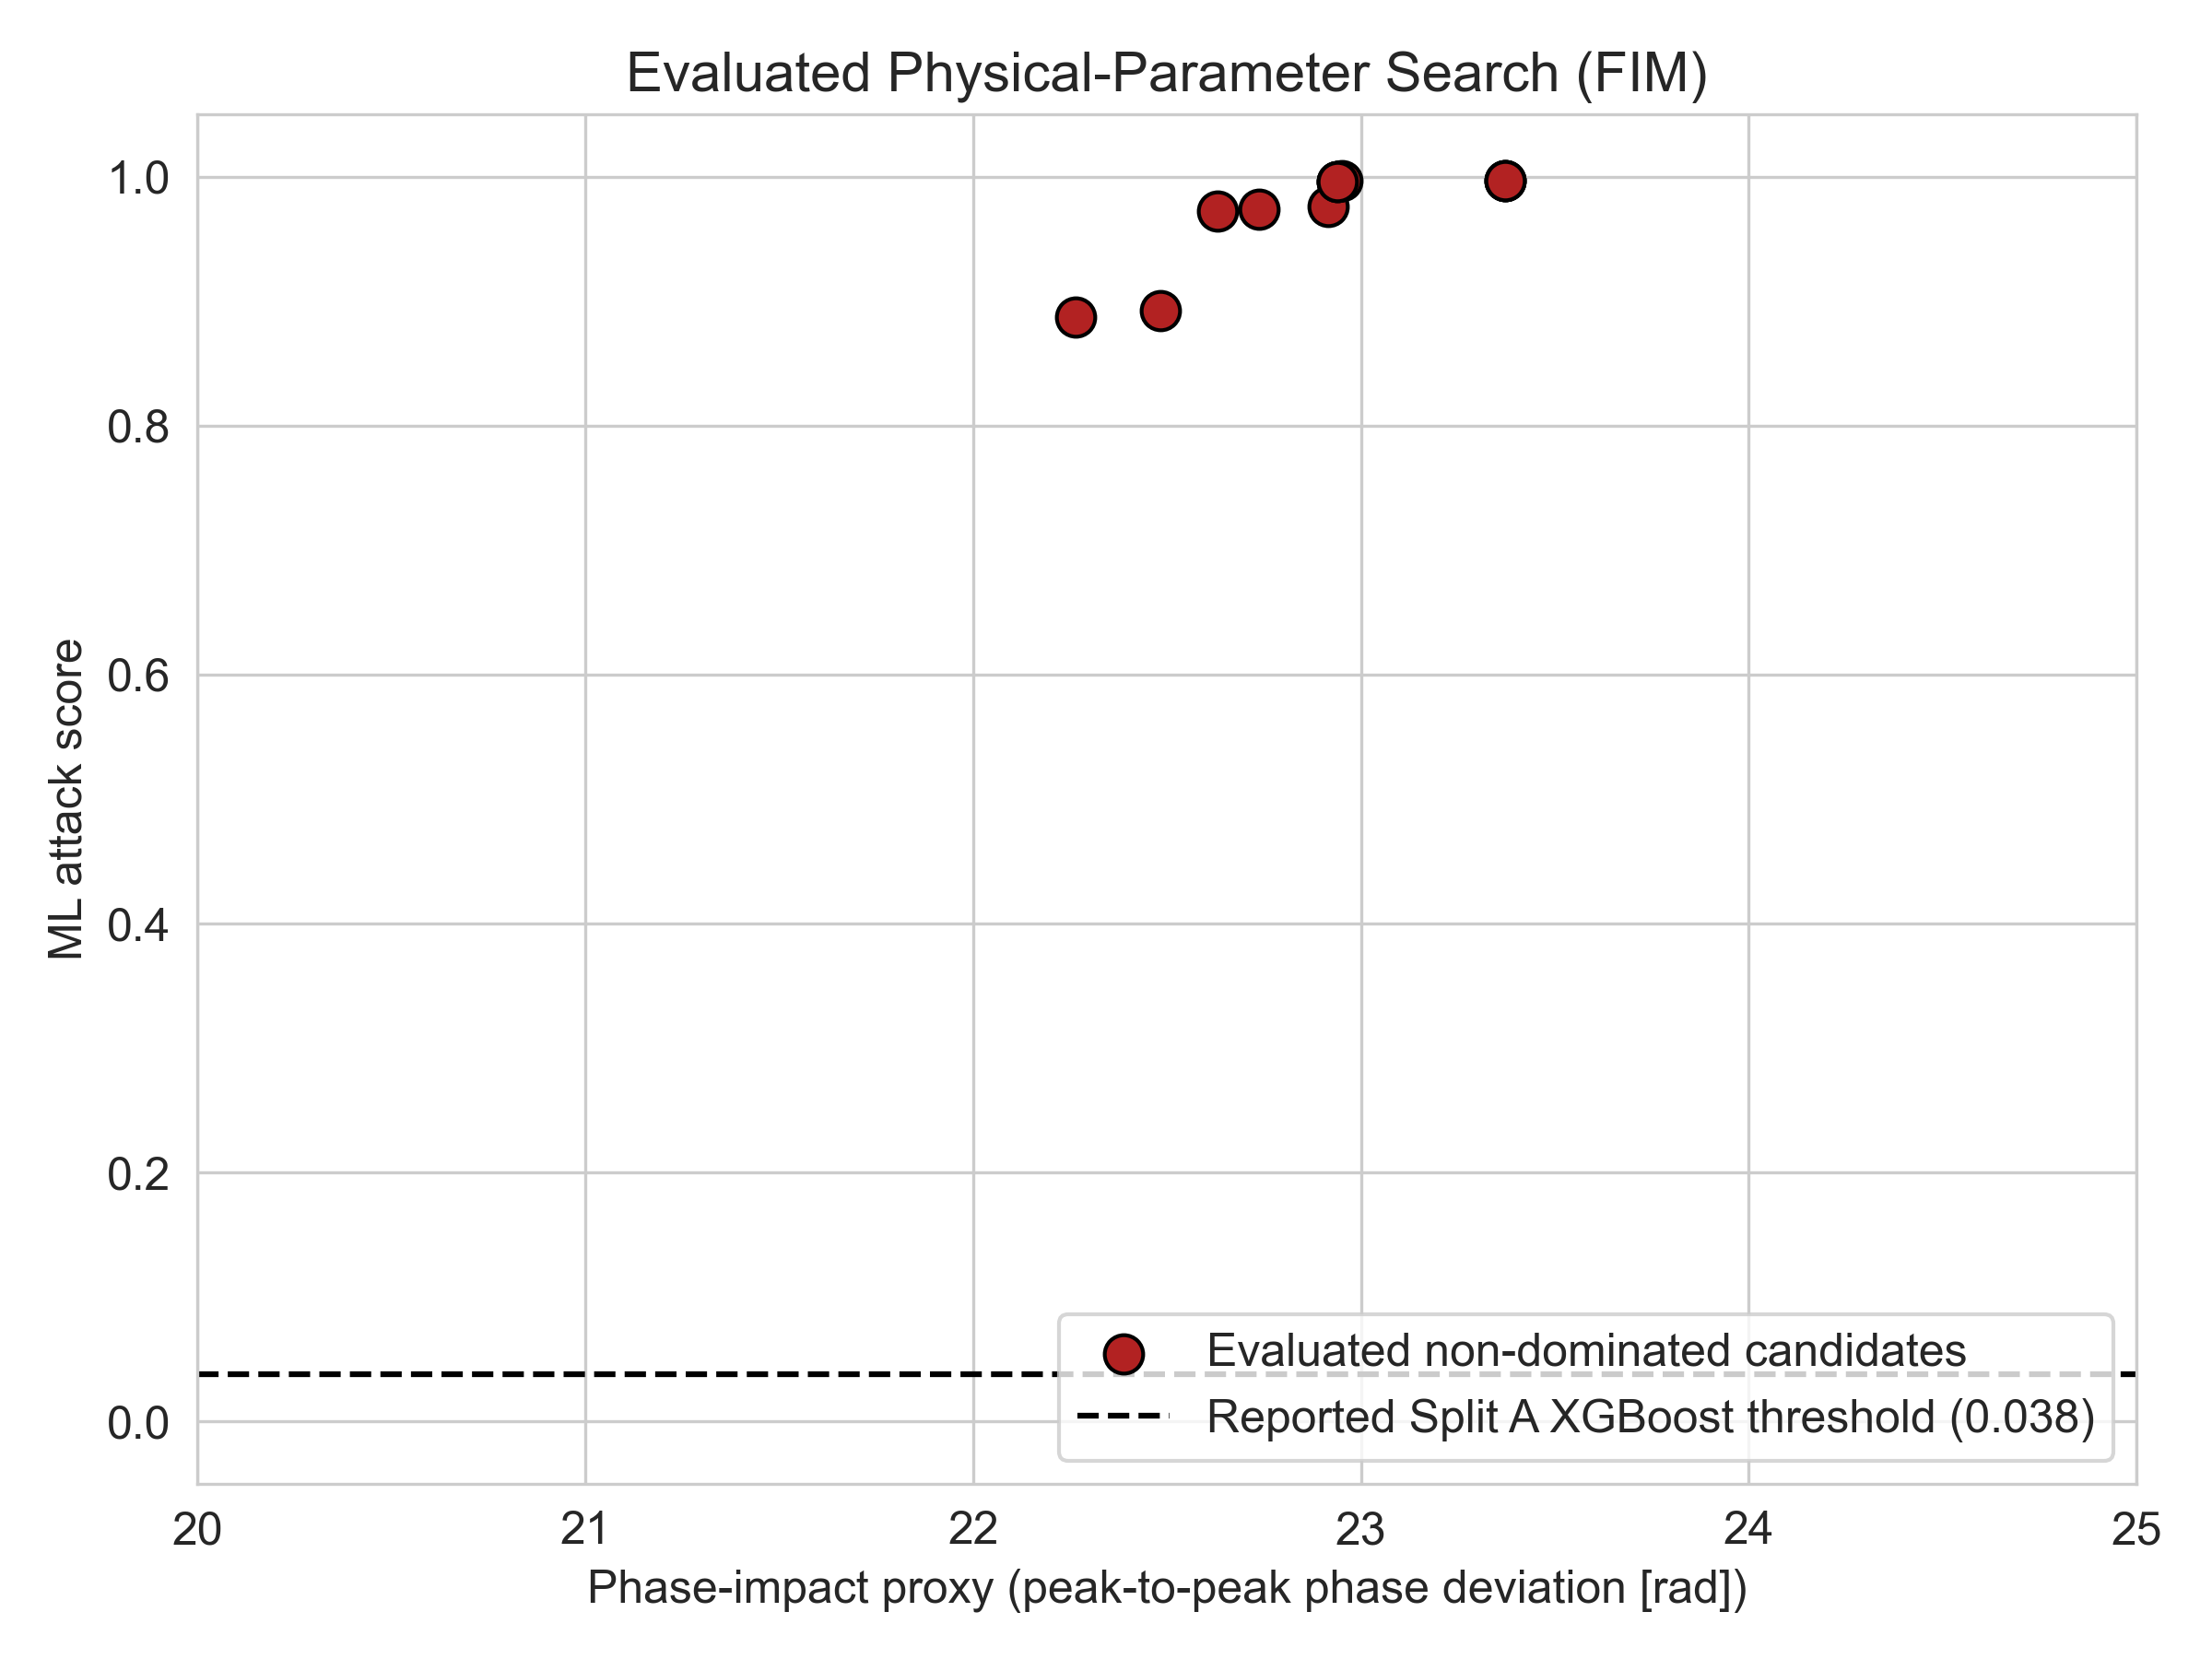
\includegraphics[width=1\linewidth]{results/figures/evasion_frontier_fim.png}
  \hfill
  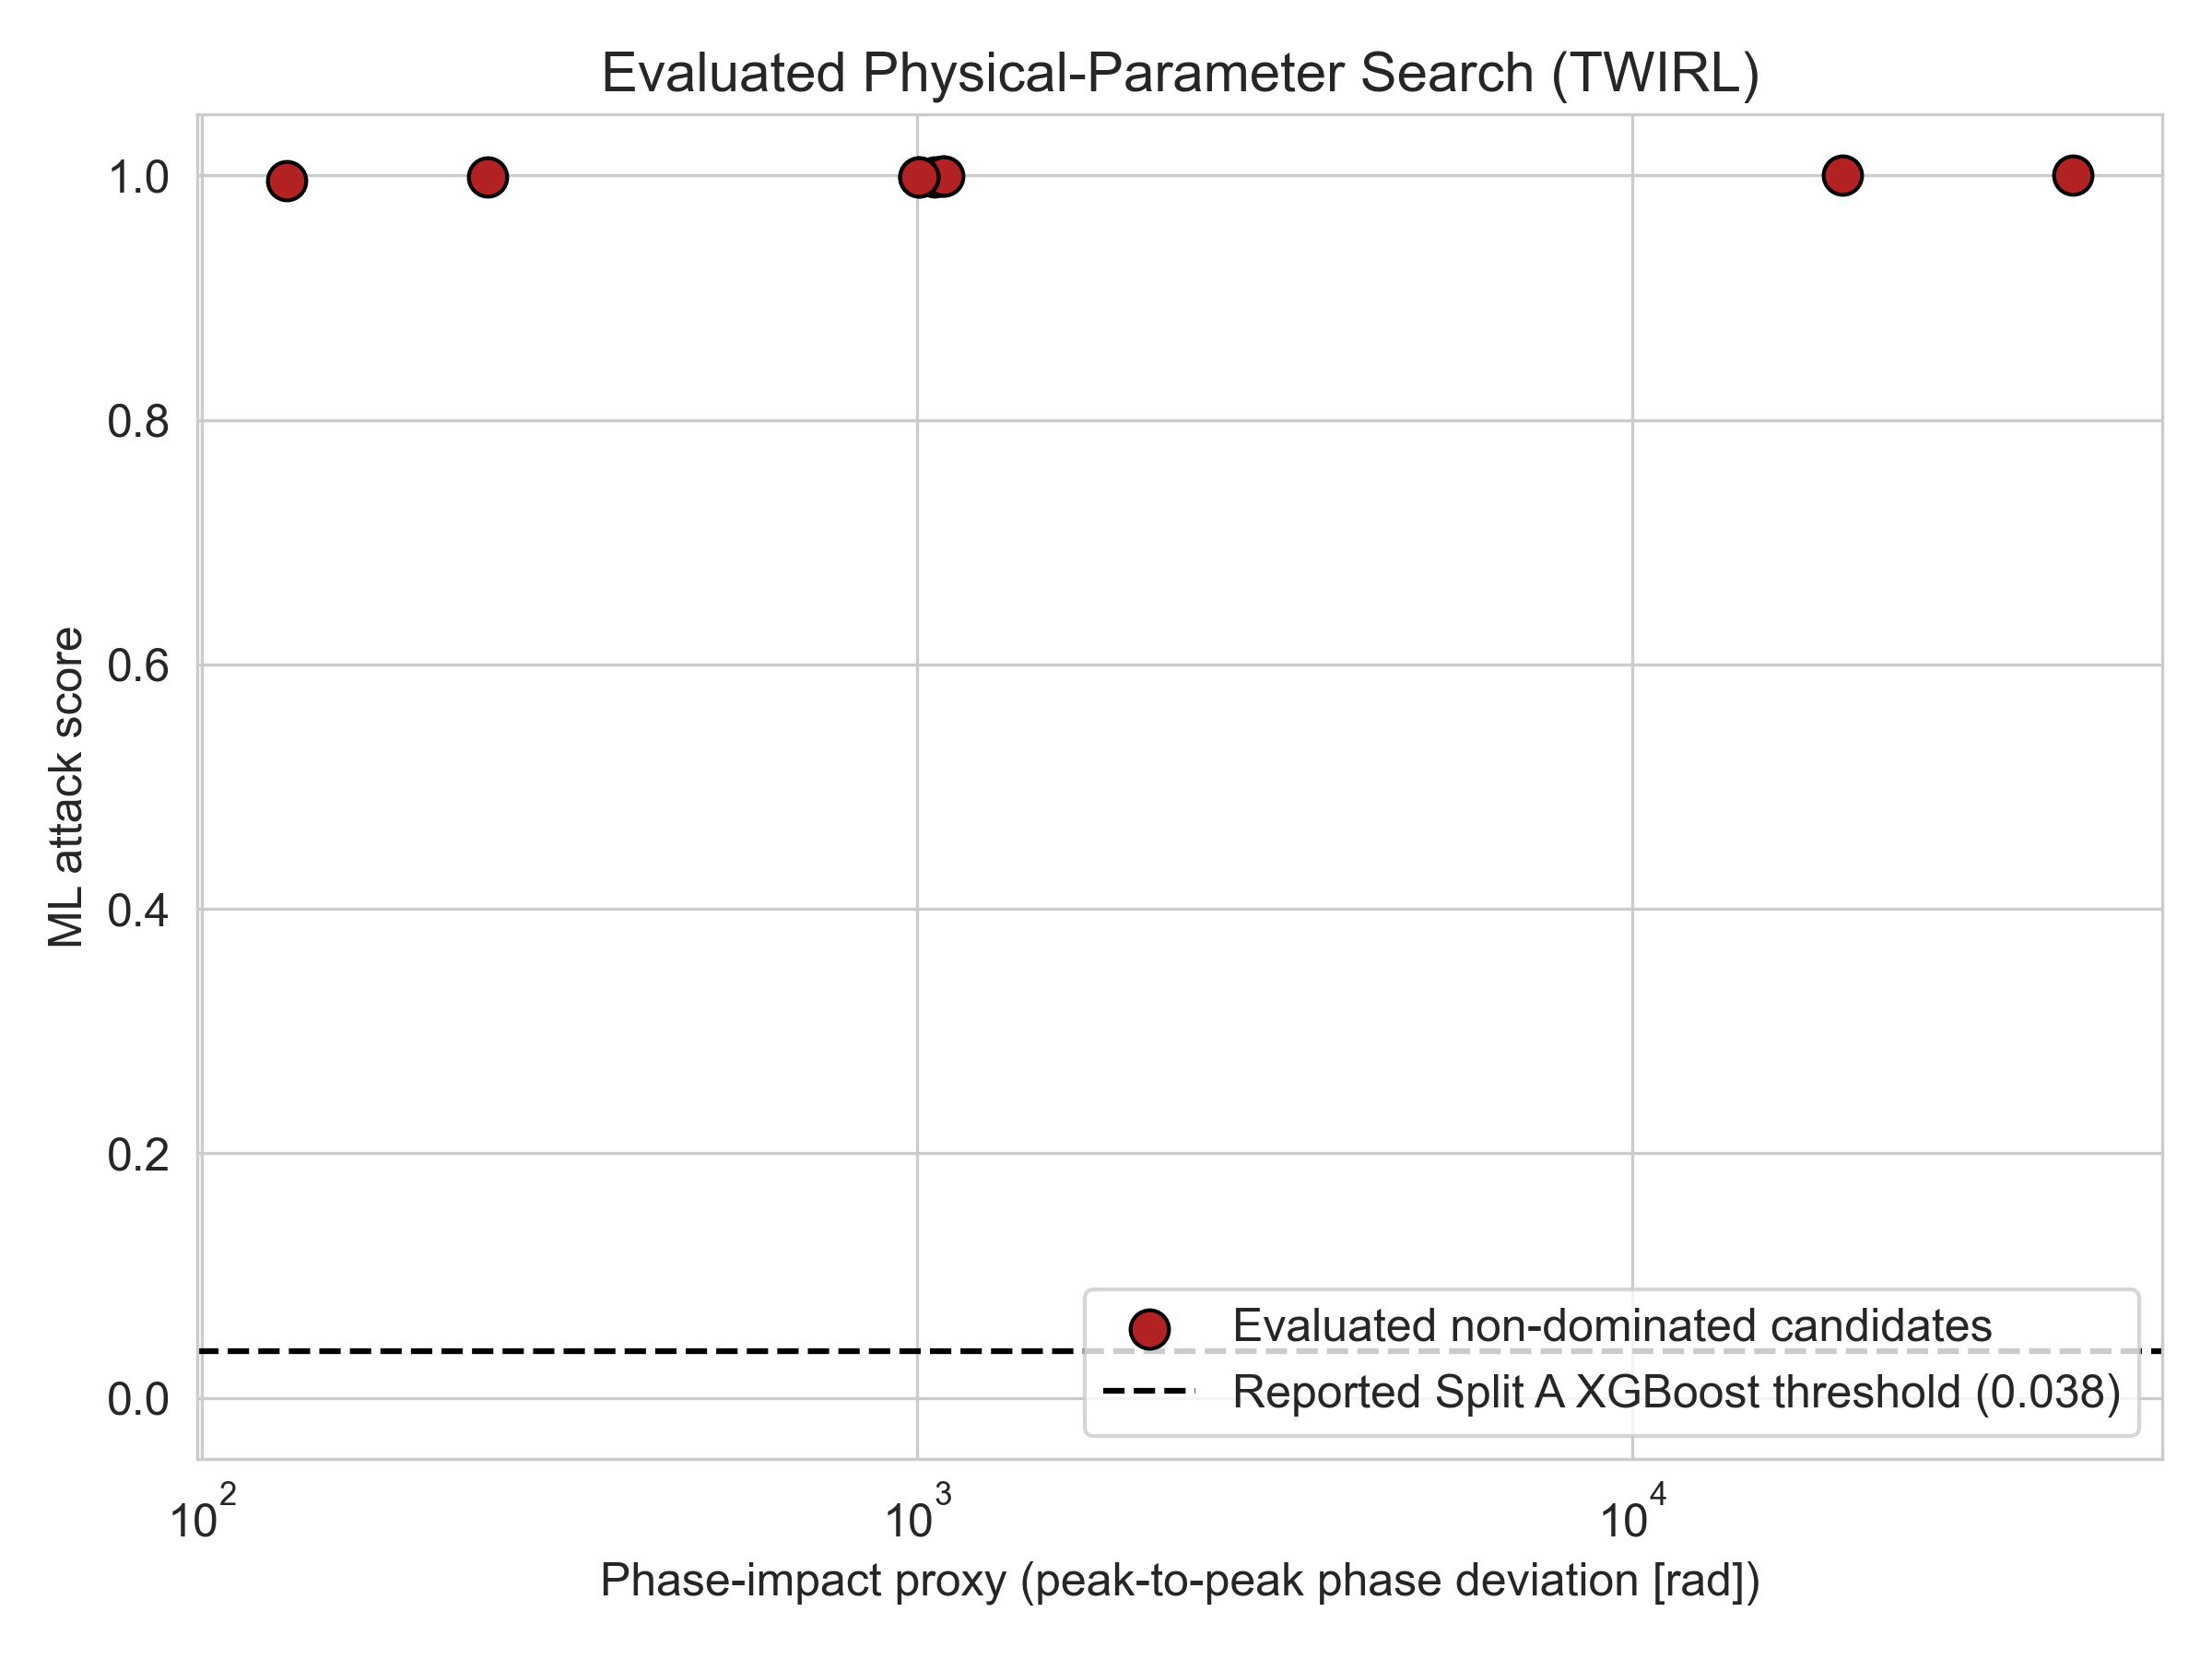
\includegraphics[width=1\linewidth]{results/figures/evasion_frontier_twirl.png}
  \caption{Evaluated optimizer candidates for FIM (upper panel) and TWIRL (lower panel).
           Each point represents a non-dominated candidate among the 200 evaluations
           for the corresponding attack family. The dashed horizontal line marks the
           reported Split A XGBoost threshold of $0.038$; attack scores do not depend
           on this threshold. Panels are stacked.}
  \label{fig:frontier}
\end{figure}

\paragraph{FIM evasion.}
Among the 200 evaluated FIM configurations, the minimum observed attack score is
$\patk^*=0.887$, attained at $m=0.103$ and
$f_\mathrm{fim}=\SI{2.91}{\giga\hertz}$. The associated phase-impact proxy is
reported as $\hobs=22.26$~rad in the current experimental record. Because this proxy
is correlated with phase-derived classifier features, this point does not establish
a trade-off against independent physical impact.

\paragraph{TWIRL evasion.}
Among the 200 evaluated TWIRL configurations, the minimum observed attack score is
$\patk^*=0.996$, reached at $\Delta\lambda=\SI{0.32}{\nano\metre}$ with
$\hobs=131.5$~rad. The evaluated TWIRL candidates remained near an attack score of
one across the reported search. Such saturated tree scores can provide little ranking
information to NSGA-II, so this single 200-evaluation run does not characterize the
score landscape or establish a lower bound over the continuous parameter domain.

\subsection{Defense Comparison}

Fig.~\ref{fig:defense} compares reported supervised-model FPR values on simulated
benign drift data. PIAD is omitted because no calibrated PIAD alarm threshold or
trajectory-level false-positive evaluation is available.

\begin{figure}[t]
  \centering
  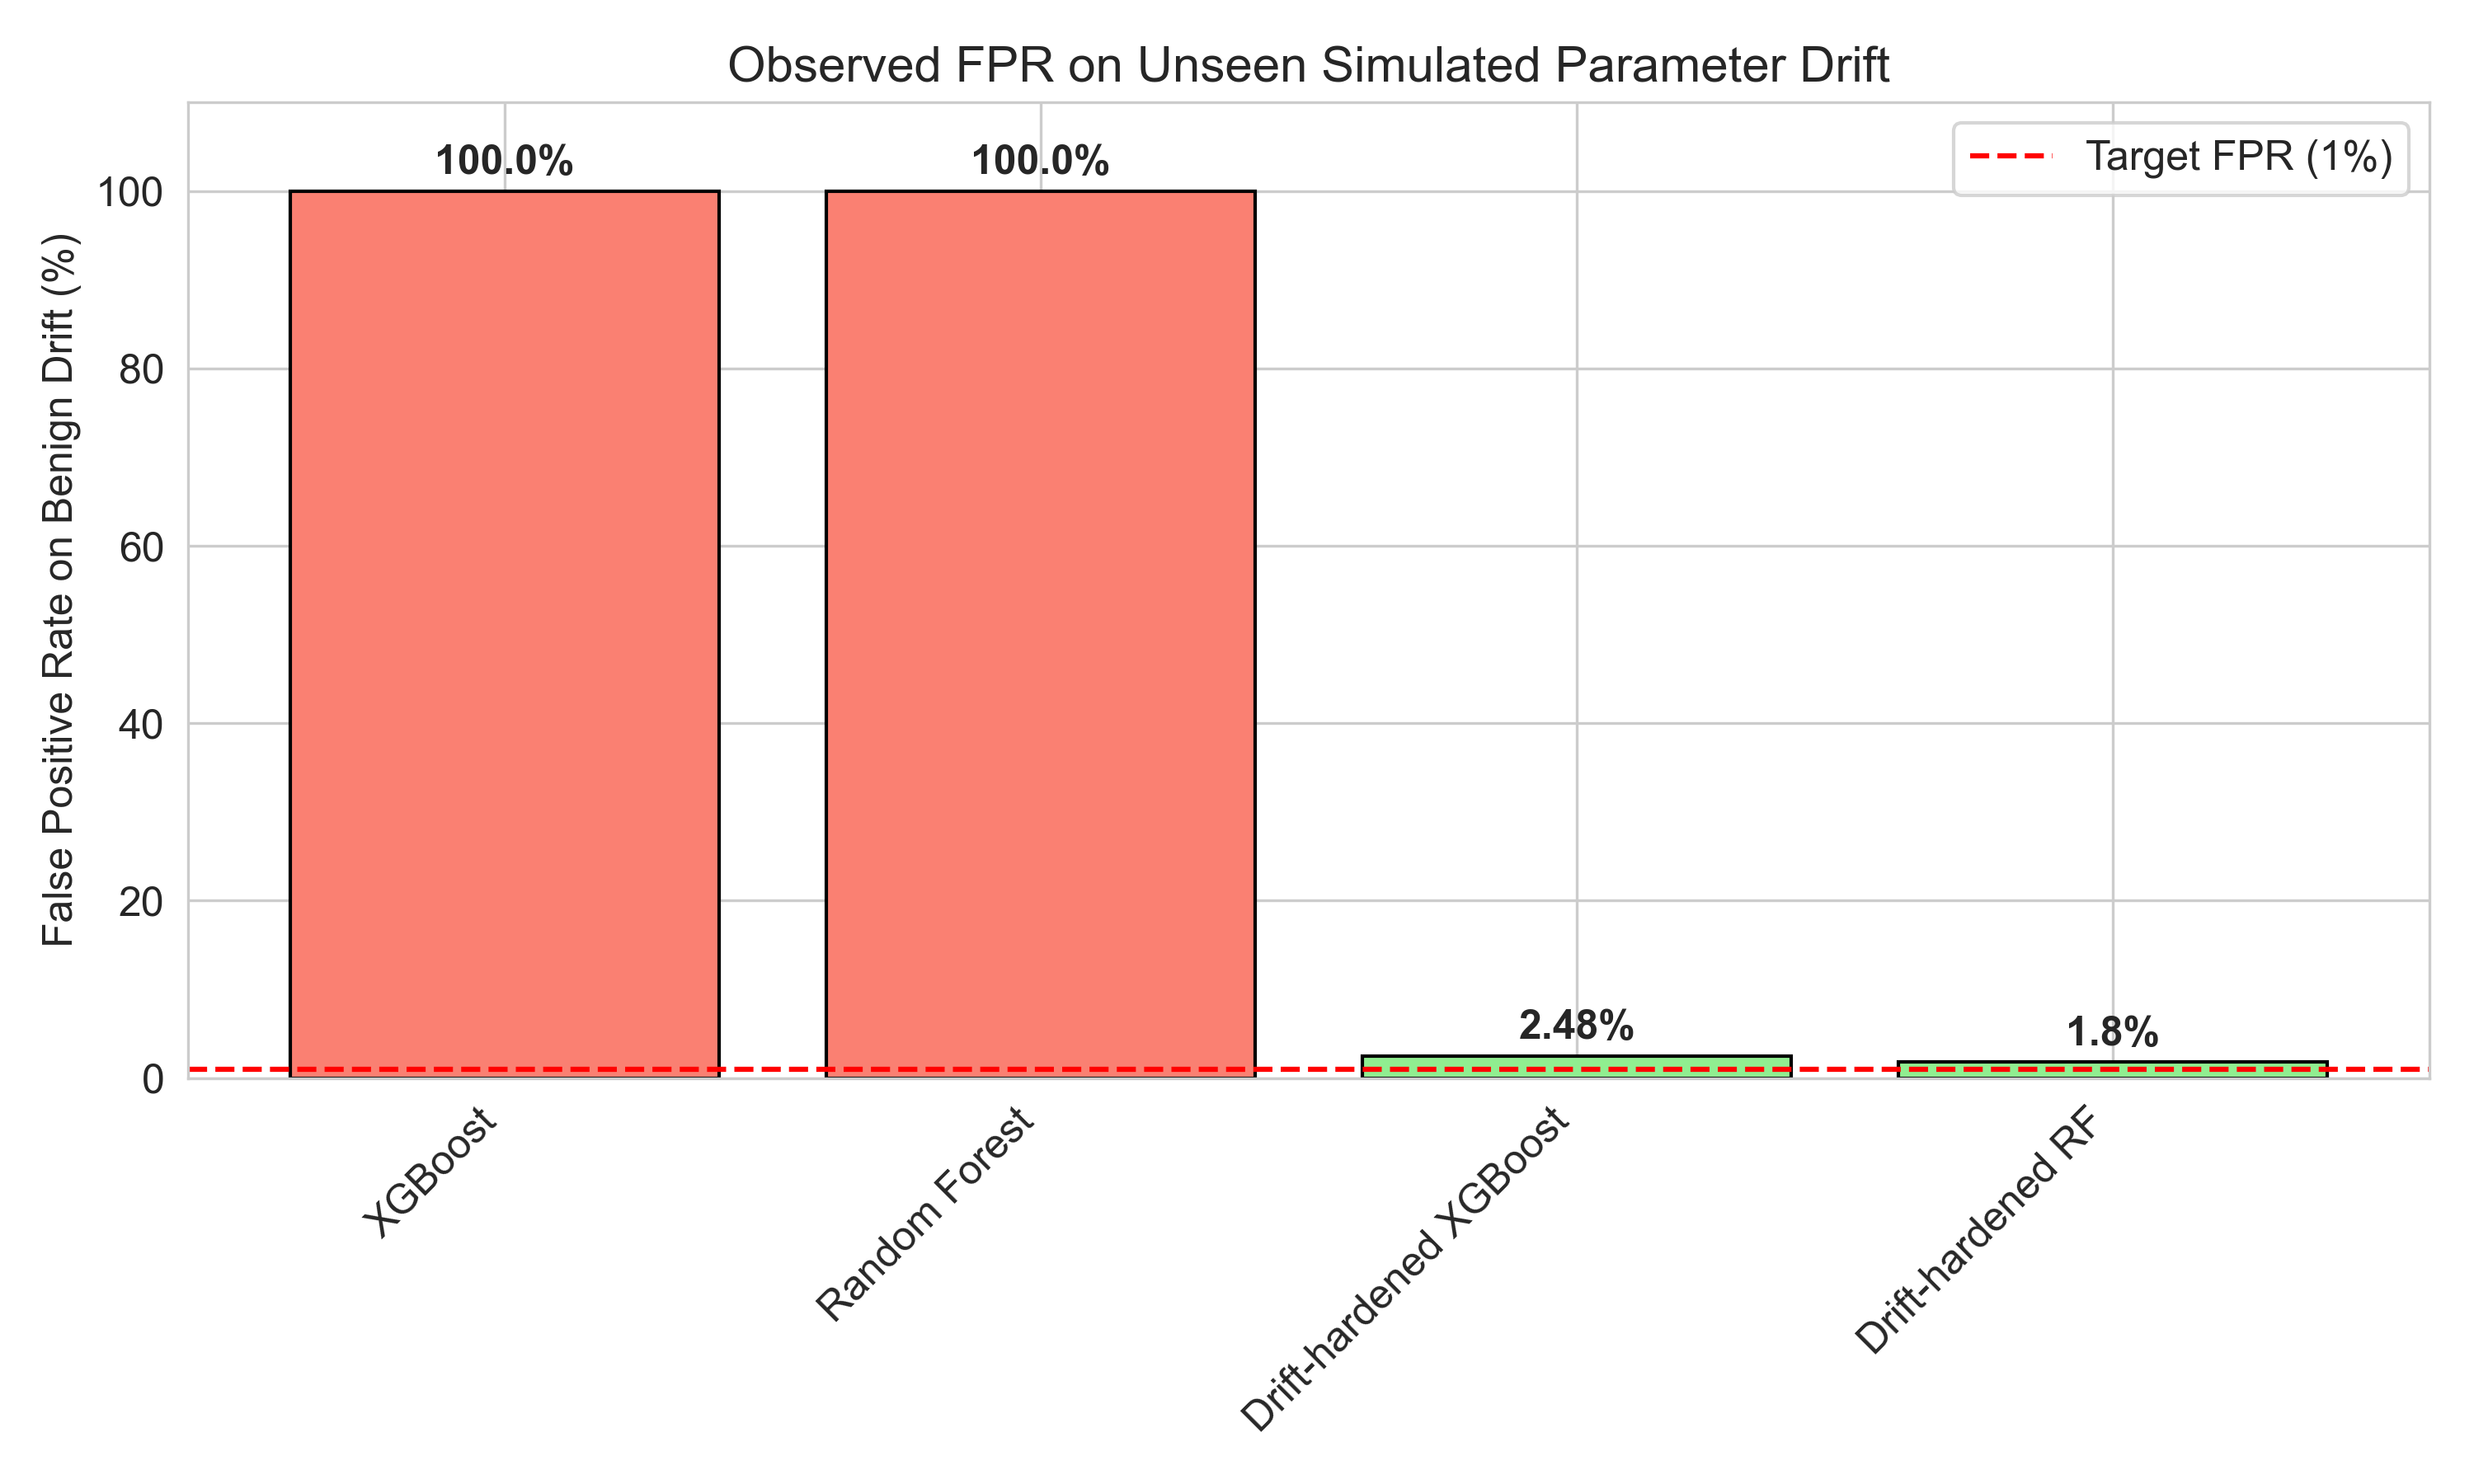
\includegraphics[width=\linewidth]{results/figures/defense_comparison.png}
  \caption{Reported false-positive rates on unseen simulated parameter drift for
           supervised models. Values are provisional pending threshold regeneration;
           PIAD is not plotted because its alarm threshold and FPR were not evaluated.}
  \label{fig:defense}
\end{figure}

Drift-hardened retraining is reported to reduce the measured FPR from $100\%$ to
approximately $2.5\%$ for XGBoost and $1.8\%$ for Random Forest, consistent with the
baseline study~\cite{basepaper}; these values require evaluation under regenerated
thresholds. The condition-level PIAD residual table does not establish an FPR, and no
combined-detector performance is reported.

% -----------------------------------------------------------------------
% IX. DISCUSSION
% -----------------------------------------------------------------------
\section{Discussion}
\label{sec:discussion}

\paragraph{On the observed adversarial frontier.}
The lowest scores among the 200 evaluated candidates remained above the reported
Split A alarm threshold. This means the search found no evasion in that candidate
set. It does not establish monitor robustness: the phase-impact proxy shares phase
information with the features, and near-saturated tree scores may give NSGA-II a
flat objective landscape. No dense grid, repeated optimizer runs, or independent
impact measure was evaluated.

\paragraph{On the monitor's brittleness under drift.}
The evaluated supervised models exhibit a $100\%$ FPR on two fixed simulated
parameter changes. Because the nominal trajectories are deterministic and contain
no measurement or phase noise, this result may reflect a degenerate nominal class;
it is not an estimate of real-device alarm rates or a drift-response curve.

\paragraph{On the PIAD's limitations.}
PIAD's reported residual floor and finite-difference construction require numerical
validation at a sampling rate that resolves the modeled dynamics, followed by noise
and bandwidth testing. Its use of the simulated carrier state $N$ also requires an
observable hardware substitute. The present condition-level means do not provide ROC,
TPR, uncertainty, or a fair comparison with nominal-only detectors using matched
inputs. PIAD does not distinguish the evaluated FIM trajectories.

\paragraph{On the phase-impact proxy.}
The phase excursion $\hobs$ is correlated with phase-derived monitor features and is
not an independent physical impact measure. Future attack searches should report
attack score subject to a prespecified phase-impact constraint and include an
amplitude- or sideband-based observable. No protocol-level security metric is
evaluated here.

\paragraph{On scope and claim boundaries.}
All results pertain exclusively to the stated numerical model. The simulated attack
parameters are grounded in~\cite{juarez2026,basepaper}, but the present study does not
validate their transfer to hardware telemetry. No claim is made regarding composable
security, finite-key performance under attack, or hardware exploitability.

\paragraph{On result status.}
Thresholds and metrics derived from thresholded decisions must be regenerated under
Eq.~\eqref{eq:threshold}. The attack scores themselves do not depend on the alarm
threshold. Split C requires disjoint groups and retraining. The implemented TWIRL
phase ramp is now stated explicitly above, but remains a simplified simulator rule,
not a physically verified wavelength conversion. Appendix~\ref{app:recalculation}
lists the remaining analysis required before circulation.

% -----------------------------------------------------------------------
% X. CONCLUSION
% -----------------------------------------------------------------------
\section{Conclusion}
\label{sec:conclusion}

This simulator study evaluated a bounded physical-parameter search, supervised
classification under two fixed simulated drift conditions, and a nominal phase
residual. In a single 200-evaluation search, the minimum observed XGBoost attack
scores were $0.887$ for FIM and $0.996$ for TWIRL, both above the reported Split A
threshold. The supervised models produced $100\%$ observed FPR on the specified
simulated drift samples. The condition-level PIAD residual matched between nominal
and tested FIM conditions, while no thresholded PIAD detection metric is available.
These results are
limited by deterministic nominal trajectories, unmodeled measurement noise, coarse
phase sampling, a phase-correlated impact proxy, a simplified TWIRL phase ramp, and
nominal-group overlap in Split C. They do not establish physical robustness or
protocol security.

Before further interpretation, Split C must be rebuilt with disjoint trajectory
groups and all threshold-dependent metrics regenerated with trajectory-level
uncertainty. The simulator evaluation also needs stochastic measurement and phase
noise, drift-magnitude sweeps, noise-resolved PIAD baselines, an independent
amplitude-based impact measure, and an attack search over a dense parameter grid.
Hardware validation and a later protocol-level analysis remain necessary.

% -----------------------------------------------------------------------
% REPRODUCIBILITY CHECKLIST
% -----------------------------------------------------------------------
\appendix
\section{Results-Recalculation and Implementation Checklist}
\label{app:recalculation}

The following items remain before the numerical results can support the broader
claims considered in this manuscript.
\begin{enumerate}
  \item Regenerate each validation threshold using Eq.~\eqref{eq:threshold}, then
        recompute threshold-dependent validation/test FPR, FNR, class recalls, and
        all corresponding tables and figures. Record the threshold comparison
        convention. The candidate attack scores in Section~\ref{sec:attack} do not
        depend on this threshold and need not be recomputed for this correction.
  \item Correct Split C so that no trajectory group appears in both partitions,
        retrain each model, and replace its current metrics. The current Split C
        numbers are not valid held-out estimates.
  \item Add trajectory-clustered uncertainty intervals, repeat model training across
        seeds, and report the number of independent nominal and drift trajectories.
        Evaluate FPR across drift magnitudes and test drift-hardening on held-out
        drift conditions.
  \item Add physically motivated stochastic and measurement noise, verify the PIAD
residual at a sampling rate that resolves the modeled dynamics, define and calibrate
a nominal threshold on held-out trajectories, decompose
        its residual by term, and compare ROC/TPR against nominal-only baselines using
        matched observable inputs. Include noise and bandwidth sweeps.
  \item Replace or supplement the phase-correlated impact proxy with an
        amplitude- or sideband-based measure. Evaluate a dense FIM grid and TWIRL
        sweep, report score subject to a stated impact constraint, and assess search
        variability across repeated optimizer runs.
  \item Treat the TWIRL phase ramp as a simplified simulator rule unless a physically
        justified wavelength-to-frequency and locking response is implemented.
        Document the reference wavelength, injected field amplitude, power ratio,
        initial conditions, and units for every attack input.
  \item Verify that every table, plot, and narrative value matches the regenerated
        artifacts; record code revision, random seeds, split identifiers, and
        evaluation settings. Report confidence intervals at the trajectory level,
        not by treating correlated windows as independent samples.
  \item Confirm authorship and acknowledgment with T.~S.~L.~Radhika, whose work is
        the basis for the simulator and baseline framework, before circulating the
        manuscript.
\end{enumerate}

Until these steps are complete, the current results should be described as
exploratory observations from the specified deterministic simulator.

% -----------------------------------------------------------------------
% ACKNOWLEDGMENT
% -----------------------------------------------------------------------
\section*{Acknowledgment}

The author thanks the faculty of the Department of Physics and Electronics \&
Electrical Engineering, BITS Pilani Hyderabad Campus, for guidance and access to
computational resources. The experimental reference-beam attack measurements that
ground the threat model of this work were reported by Juárez~\emph{et~al.}~\cite{juarez2026}.
The baseline ML detection framework and open-source simulator used as the starting
point for this study were developed in~\cite{basepaper}.

% -----------------------------------------------------------------------
% BIBLIOGRAPHY
% -----------------------------------------------------------------------
\begin{thebibliography}{99}

\bibitem{lucamarini2018}
M.~Lucamarini, Z.~L.~Yuan, J.~F.~Dynes, and A.~J.~Shields,
``Overcoming the rate-distance limit of quantum key distribution without
quantum repeaters,''
\emph{Nature}, vol.~557, pp.~400--403, May 2018.

\bibitem{wang2018}
X.-B.~Wang, Z.-W.~Yu, and X.-L.~Hu,
``Twin-field quantum key distribution with large misalignment error,''
\emph{Phys. Rev. A}, vol.~98, p.~062323, Dec. 2018.

\bibitem{pirandola2020}
S.~Pirandola \emph{et~al.},
``Advances in quantum cryptography,''
\emph{Adv. Opt. Photon.}, vol.~12, pp.~1012--1236, 2020.

\bibitem{roberts2017}
G.~L.~Roberts \emph{et~al.},
``Patterning-effect mitigating intensity modulator for secure high-speed
quantum key distribution,''
\emph{Opt. Lett.}, vol.~42, pp.~4613--4616, 2017.

\bibitem{juarez2026}
S.~Juárez \emph{et~al.},
``Reference-beam attacks against twin-field quantum key distribution using
optical injection locking,''
\emph{Phys. Rev. A}, vol.~113, no.~3, p.~032613, 2026.

\bibitem{basepaper}
M.~H.~Astik and T.~S.~L.~Radhika,
``ML-based attack detection for twin-field QKD with optical injection locking,''
in \emph{Proc. 2026 International Conference on Intelligent Computing and Secure
Communication Systems (ICICSCS)}, 2026. [Online]. Available:
\url{https://github.com/lihtim-kitsa/ml-attack-detection-tfqkd-oil}

\bibitem{baliuka2023}
A.~Baliuka, M.~Stöcker, M.~Auer, P.~Freiwang, H.~Weinfurter, and L.~Knips,
``Deep-learning-based radio-frequency side-channel attack on quantum key distribution,''
\emph{Phys. Rev. Applied}, vol.~20, no.~5, p.~054040, 2023.

\bibitem{almohammed2021}
H.~A.~Al-Mohammed \emph{et~al.},
``Machine learning techniques for detecting attackers during quantum key distribution
in IoT networks with application to railway scenarios,''
\emph{IEEE Access}, vol.~9, pp.~136994--137004, 2021.

\bibitem{tunc2023}
H.~S.~D.~Tunc, Y.~Wang, R.~Bassoli, and F.~H.~Fitzek,
``Machine learning based attack detection for quantum key distribution,''
in \emph{Proc. IEEE 9th World Forum on Internet of Things (WF-IoT)}, 2023, pp.~1--6.

\bibitem{du2022}
H.~Du and D.~Huang,
``Multi-attack detection: General defense strategy based on neural networks for CV-QKD,''
\emph{Photonics}, vol.~9, no.~3, p.~177, 2022.

\bibitem{luo2022}
H.~Luo \emph{et~al.},
``Beyond universal attack detection for continuous-variable quantum key distribution via
deep learning,''
\emph{Phys. Rev. A}, vol.~105, no.~4, p.~042411, 2022.

\bibitem{ding2023mads}
C.~Ding, S.~Wang, Y.~Wang, Z.~Wu, J.~Sun, and Y.~Mao,
``Machine-learning-based detection for quantum hacking attacks on continuous-variable
quantum-key-distribution systems,''
\emph{Phys. Rev. A}, vol.~107, no.~6, p.~062422, 2023.

\bibitem{xu2024mlqkd}
J.~Xu \emph{et~al.},
``Automatically identifying imperfections and attacks in practical quantum key
 distribution systems via machine learning,''
\emph{Sci. China Inf. Sci.}, vol.~67, no.~10, p.~202501, 2024.

\bibitem{liu2025}
J.~Liu, B.~Huang, J.~Su, Q.~Peng, and A.~Huang,
``Deep anomaly detection for active attacks on the receiver in quantum key distribution,''
\emph{Opt. Express}, vol.~33, no.~22, pp.~47137--47150, 2025.

\bibitem{deng2017}
R.~Deng \emph{et~al.},
``False data injection on state estimation in power systems---attacks, impacts,
and defense: A survey,''
\emph{IEEE Trans. Ind. Inform.}, vol.~13, pp.~411--423, Apr. 2017.

\bibitem{papernot2016}
N.~Papernot, P.~McDaniel, S.~Jha, M.~Fredrikson, Z.~B.~Celik, and A.~Swami,
``The limitations of deep learning in adversarial settings,''
in \emph{Proc. IEEE Eur. Symp. Secur. Privacy (EuroS\&P)}, Saarbrücken, Germany,
2016, pp.~372--387.

\bibitem{peng2023}
Z.~Peng, Y.~Jiang, and C.~Guo,
``Machine learning for optical performance monitoring in coherent optical systems,''
\emph{J. Lightw. Technol.}, vol.~41, no.~3, pp.~912--923, 2023.

\bibitem{lang1980}
R.~Lang and K.~Kobayashi,
``External optical feedback effects on semiconductor injection laser properties,''
\emph{IEEE J. Quantum Electron.}, vol.~QE-16, no.~3, pp.~347--355, 1980.

\bibitem{raissi2019}
M.~Raissi, P.~Perdikaris, and G.~E.~Karniadakis,
``Physics-informed neural networks: A deep learning framework for solving forward
and inverse problems involving nonlinear partial differential equations,''
\emph{J. Comput. Phys.}, vol.~378, pp.~686--707, 2019.

\bibitem{cai2021}
S.~Cai, Z.~Mao, Z.~Wang, M.~Yin, and G.~E.~Karniadakis,
``Physics-informed neural networks (PINNs) for fluid mechanics: A review,''
\emph{Acta Mech. Sin.}, vol.~37, pp.~1727--1738, 2021.

\bibitem{ritto2021}
T.~G.~Ritto and S.~Rochinha,
``Digital twin, physics-based model, and machine learning applied to monitoring
and prognosis in a lathe,''
\emph{Mech. Syst. Signal Process.}, vol.~161, p.~107967, 2021.

\bibitem{chen2018}
R.~T.~Q.~Chen, Y.~Rubanova, J.~Bettencourt, and D.~Duvenaud,
``Neural ordinary differential equations,''
in \emph{Adv. Neural Inf. Process. Syst. (NeurIPS)}, vol.~31, 2018,
pp.~6571--6583.

\bibitem{chen2016xgboost}
T.~Chen and C.~Guestrin,
``XGBoost: A scalable tree boosting system,''
in \emph{Proc. 22nd ACM SIGKDD Int. Conf. Knowledge Discovery and Data Mining},
2016, pp.~785--794.

\bibitem{tomamichel2012}
M.~Tomamichel, C.~C.~W.~Lim, N.~Gisin, and R.~Renner,
``Tight finite-key analysis for quantum cryptography,''
\emph{Nature Communications}, vol.~3, p.~634, 2012.

\bibitem{jiang2019}
C.~Jiang, Z.-W.~Yu, X.-L.~Hu, and X.-B.~Wang,
``Unconditional security of sending or not sending twin-field quantum key distribution
with finite pulses,''
\emph{Phys. Rev. Applied}, vol.~12, no.~2, p.~024061, 2019.

\bibitem{cardenas2011}
A.~A.~C\'ardenas, S.~Amin, Z.-S.~Lin, Y.-L.~Huang, C.-Y.~Huang, and S.~Sastry,
"Attacks against process control systems: Risk assessment, detection, and response,"
in \emph{Proc. 6th ACM Symp. on Information, Computer and Communications Security},
2011, pp.~355--366, doi: 10.1145/1966913.1966959.

\bibitem{urbina2016}
D.~I.~Urbina, J.~Giraldo, A.~A.~C\'ardenas, N.~O.~Tippenhauer, J.~Valente,
M.~Faisal, J.~Ruths, R.~Candell, and H.~Sandberg,
"Limiting the impact of stealthy attacks on industrial control systems,"
in \emph{Proc. 23rd ACM Conf. on Computer and Communications Security},
2016, doi: 10.1145/2976749.2978388.

\bibitem{chowdhury2020}
N.~R.~Chowdhury, J.~Belikov, D.~Baimel, and Y.~Levron,
"Observer-based detection and identification of sensor attacks in networked CPSs,"
\emph{Automatica}, vol.~121, p.~109166, 2020,
doi: 10.1016/j.automatica.2020.109166.

\bibitem{tramer2020}
F.~Tramer, N.~Carlini, W.~Brendel, and A.~Madry,
"On adaptive attacks to adversarial example defenses,"
in \emph{Adv. Neural Inf. Process. Syst.}, vol.~33, 2020.

\end{thebibliography}

\end{document}
